\documentclass[tikz,border=5pt]{standalone}
\usepackage[UTF8,fontset=fandol]{ctex}
\usepackage{amsmath,amssymb}
\usetikzlibrary{arrows.meta,calc}
\tikzset{every picture/.style={>=Latex,line cap=round,line join=round,font=\small},
 steel/.style={thick,black!75}, string/.style={very thick,blue!75!black},
 guide/.style={thin,dashed,black!35}, dim/.style={<->,thin,black!65},
 force/.style={->,very thick,red!75!black}, motion/.style={->,thick,red!70!black},
 ring/.style={circle,draw=black,fill=white,inner sep=0pt,minimum size=4.5pt}}
% r=1 in all physical geometry; the auxiliary panel is translated and uniformly enlarged.
% Perturbed positions solve the three ORIGINAL normal/total-length equations, u=.03,w=0.
\def\pertXA{-1.8831690728341308}
\def\pertYA{1.9067728833679587}
\def\pertXB{1.4891366927115461}
\def\pertYB{2.1264166901809434}
\def\pertX{0.03}
\def\pertY{-0.9989504757313443}
% Pure out-of-plane snapshot, w=1 (enlarged for spatial readability).
\def\spaceXA{-2.2360679774997897}
\def\spaceYA{1.6329931618554521}
\def\spaceXB{2.2360679774997897}
\def\spaceYB{1.6329931618554521}
\def\spaceY{-0.8164965809277260}
\def\spaceW{1}
\newcommand{\basepoints}{
 \coordinate(A)at({-sqrt(3)},2);
 \coordinate(B)at({sqrt(3)},2);
 \coordinate(Pzero)at(0,-1);
 \coordinate(O)at(0,0);
}
\newcommand{\steelellipse}{\draw[steel](0,0)ellipse[x radius=3,y radius={sqrt(6)}];}
\begin{document}

% 1: The bead is INSIDE the original ellipse, not below its lowest point.
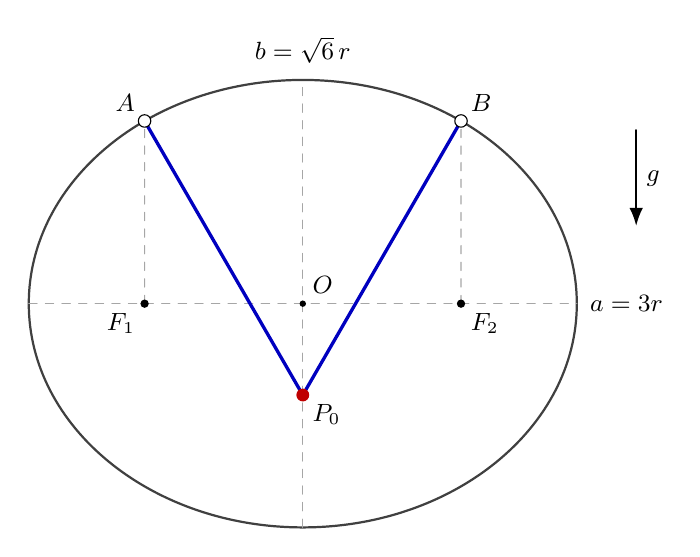
\begin{tikzpicture}[scale=1.16]
 \basepoints
 \steelellipse
 \draw[guide](-3,0)--(3,0);
 \draw[guide](0,{-sqrt(6)})--(0,{sqrt(6)});
 \draw[guide]({-sqrt(3)},0)--(A);
 \draw[guide]({sqrt(3)},0)--(B);
 \draw[string](A)--(Pzero)--(B);
 \node[ring]at(A){};
 \node[ring]at(B){};
 \fill[red!75!black](Pzero)circle(2pt);
 \fill(O)circle(1pt);
 \fill({-sqrt(3)},0)circle(1.3pt);
 \fill({sqrt(3)},0)circle(1.3pt);
 \node[above left]at(A){$A$};
 \node[above right]at(B){$B$};
 \node[below right]at(Pzero){$P_0$};
 \node[above right]at(O){$O$};
 \node[below left]at({-sqrt(3)},0){$F_1$};
 \node[below right]at({sqrt(3)},0){$F_2$};
 \node[right]at(3.04,0){$a=3r$};
 \node[above]at(0,{sqrt(6)+.08}){$b=\sqrt6\,r$};
 \draw[->,thick](3.65,1.9)--(3.65,.85)node[midway,right]{$g$};
\end{tikzpicture}

% 2: Local ring reaction opposes inward tension; bead tensions point toward A and B.
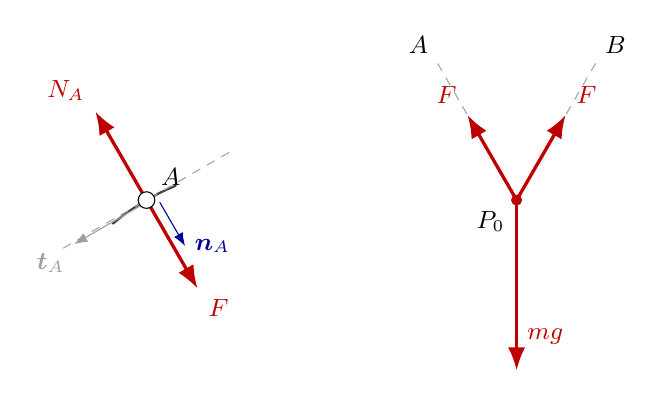
\begin{tikzpicture}
 \begin{scope}
  \draw[steel,domain=117:136,samples=60,variable=\t]
   plot({3*cos(\t)+sqrt(3)},{sqrt(6)*sin(\t)-2});
  \draw[guide]({-.866*1.22},{-.5*1.22})--({.866*1.22},{.5*1.22});
  \draw[->,thin,gray!75](-.02,-.04)--(-.92,-.56)
   node[below left]{$\boldsymbol t_A$};
  \draw[force](0,0)--(.65,-1.12583)node[below right]{$F$};
  \draw[force](0,0)--(-.65,1.12583)node[above left]{$N_A$};
  \node[ring,minimum size=6pt]at(0,0){};
  \node[above right]at(.06,.06){$A$};
  \draw[->,thin,blue!60!black](.17,-.03)--(.49,-.584)
   node[right]{$\boldsymbol n_A$};
 \end{scope}
 \begin{scope}[xshift=4.7cm]
  \draw[guide](0,0)--(-1.0,1.73205);
  \draw[guide](0,0)--(1.0,1.73205);
  \draw[force](0,0)--(-.625,1.08253)node[above left]{$F$};
  \draw[force](0,0)--(.625,1.08253)node[above right]{$F$};
  \draw[force](0,0)--(0,-2.16506)node[pos=.8,right]{$mg$};
  \fill[red!75!black](0,0)circle(2pt);
  \node[below left]at(-.03,-.02){$P_0$};
  \node[above left]at(-1.0,1.73205){$A$};
  \node[above right]at(1.0,1.73205){$B$};
 \end{scope}
\end{tikzpicture}

% 3: Osculating arcs are local. Correct order is A--O1--P0 and B--O2--P0.
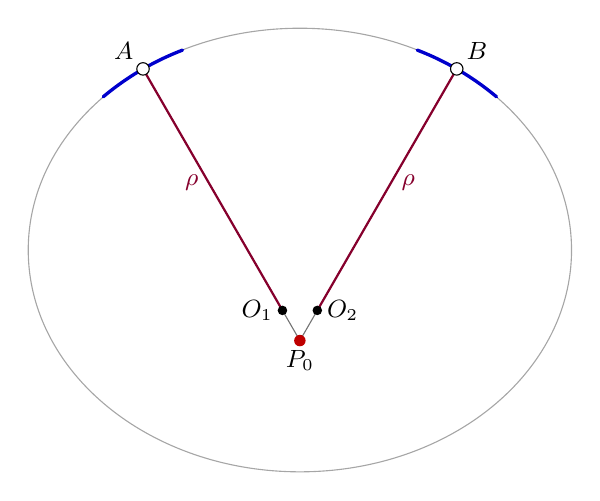
\begin{tikzpicture}[scale=1.15]
 \basepoints
 \coordinate(Oone)at({-1/(3*sqrt(3))},{-2/3});
 \coordinate(Otwo)at({1/(3*sqrt(3))},{-2/3});
 \draw[thin,black!35](0,0)ellipse[x radius=3,y radius={sqrt(6)}];
 \draw[thin,black!55](A)--(Pzero)--(B);
 \draw[blue!80!black,very thick,domain=111:130,samples=50,variable=\t]
  plot({-1/(3*sqrt(3))+16/(3*sqrt(3))*cos(\t)},
       {-2/3+16/(3*sqrt(3))*sin(\t)});
 \draw[blue!80!black,very thick,domain=50:69,samples=50,variable=\t]
  plot({1/(3*sqrt(3))+16/(3*sqrt(3))*cos(\t)},
       {-2/3+16/(3*sqrt(3))*sin(\t)});
 \draw[purple!70!black,thick](Oone)--(A)
  node[pos=.53,left]{$\rho$};
 \draw[purple!70!black,thick](Otwo)--(B)
  node[pos=.53,right]{$\rho$};
 \node[ring]at(A){};
 \node[ring]at(B){};
 \fill(Oone)circle(1.5pt);
 \fill(Otwo)circle(1.5pt);
 \fill[red!75!black](Pzero)circle(1.8pt);
 \node[above left]at(A){$A$};
 \node[above right]at(B){$B$};
 \node[left]at(Oone){$O_1$};
 \node[right]at(Otwo){$O_2$};
 \node[below]at(Pzero){$P_0$};
\end{tikzpicture}

% 4: Uniform zoom of the LOCAL auxiliary ellipse, origin at its center C_*.
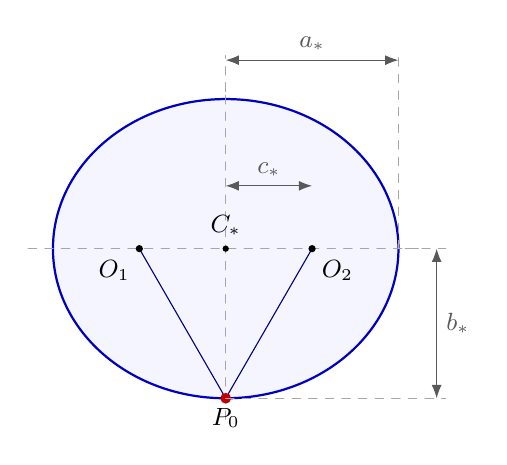
\begin{tikzpicture}[scale=5.7]
 \def\ae{0.3849001794597505}
 \def\ce{0.1924500897298753}
 \def\be{0.3333333333333333}
 \fill[blue!4](0,0)ellipse[x radius=\ae,y radius=\be];
 \draw[blue!75!black,thick](0,0)ellipse[x radius=\ae,y radius=\be];
 \draw[guide](-.44,0)--(.44,0);
 \draw[guide](0,-.38)--(0,.37);
 \draw[thin,blue!50!black](-\ce,0)--(0,-\be)--(\ce,0);
 \fill(-\ce,0)circle(.23pt);
 \fill(\ce,0)circle(.23pt);
 \fill(0,0)circle(.20pt);
 \fill[red!75!black](0,-\be)circle(.34pt);
 \node[below left]at(-\ce,-.005){$O_1$};
 \node[below right]at(\ce,-.005){$O_2$};
 \node[above]at(0,.008){$C_*$};
 \node[below]at(0,-\be){$P_0$};
 \draw[guide](0,.35)--(0,.43);
 \draw[guide](\ae,0)--(\ae,.43);
 \draw[dim](0,.42)--(\ae,.42)node[midway,above]{$a_*$};
 \draw[guide](.40,0)--(.49,0);
 \draw[guide](0,-\be)--(.49,-\be);
 \draw[dim](.47,0)--(.47,-\be)node[midway,right]{$b_*$};
 \draw[dim](0,.14)--(\ce,.14)node[midway,above]{$c_*$};
\end{tikzpicture}

% 5: Exact finite snapshot from original constraints; small bead displacement shown in uniform zoom.
\begin{tikzpicture}[scale=1.12]
 \basepoints
 \coordinate(Ap)at(\pertXA,\pertYA);
 \coordinate(Bp)at(\pertXB,\pertYB);
 \coordinate(Pp)at(\pertX,\pertY);
 \steelellipse
 \draw[guide](A)--(Pzero)--(B);
 \draw[string](Ap)--(Pp)--(Bp);
 \node[ring,draw=black!35]at(A){};
 \node[ring,draw=black!35]at(B){};
 \node[ring,draw=red!75!black]at(Ap){};
 \node[ring,draw=red!75!black]at(Bp){};
 \fill[red!75!black](Pp)circle(1.6pt);
 \node[above left]at(Ap){$A'$};
 \node[above left]at(Bp){$B'$};
 \node[right]at({sqrt(3)+.08},2){$B$};
 \node[right]at({-sqrt(3)+.06},2){$A$};
 % arrows are along each physical curve, offset outward only to avoid covering the rings.
 \draw[motion,domain=54.73561:60.23928,samples=30,variable=\t]
  plot({3.5*cos(\t)},{2.95*sin(\t)});
 \draw[motion,domain=125.26439:128.88459,samples=30,variable=\t]
  plot({3.5*cos(\t)},{2.95*sin(\t)});
 \draw[thin,gray](Pp)--(1.4,-1.6)--(3.55,-1.6);
 \begin{scope}[shift={(4.05,-1.02)}]
  \node[above]at(1.05,.70){质点附近（放大）};
  \draw[thin,gray!70](-.18,0)--(2.20,0);
  \coordinate(pz)at(0,0);
  \coordinate(pp)at({50*\pertX},{50*(\pertY+1)});
  \draw[->,thin,red!70!black](pz)--(pp);
  \fill(pz)circle(1.3pt);
  \fill[red!75!black](pp)circle(1.6pt);
  \node[above left]at(pz){$P_0$};
  \node[above right]at(pp){$P'$};
  \draw[guide](0,-.10)--(0,-.34);
  \draw[guide]({50*\pertX},0)--({50*\pertX},-.34);
  \draw[->,thin](0,-.28)--({50*\pertX},-.28)
   node[midway,below]{$u>0$};
 \end{scope}
\end{tikzpicture}

% 6: Orthographic 3D projection: vertical steel plane xy, visible out-of-plane w direction.
\begin{tikzpicture}[x={(.64278761cm,.38302222cm)},y={(0cm,.86602540cm)},
 z={(.76604444cm,-.32139380cm)},scale=1.18]
 \coordinate(As)at(\spaceXA,\spaceYA,0);
 \coordinate(Bs)at(\spaceXB,\spaceYB,0);
 \coordinate(Ps)at(0,\spaceY,\spaceW);
 \coordinate(Ppr)at(0,\spaceY,0);
 \fill[gray!5](-3.45,-2.78,0)--(3.45,-2.78,0)--(3.45,2.78,0)--(-3.45,2.78,0)--cycle;
 \draw[guide](-3.45,-2.78,0)--(3.45,-2.78,0)--(3.45,2.78,0)--(-3.45,2.78,0)--cycle;
 \draw[steel,domain=0:360,samples=180,variable=\t]
  plot({3*cos(\t)},{sqrt(6)*sin(\t)},0);
 \draw[->,thin,gray!60](0,0,0)--(3.9,0,0)node[right]{$x$};
 \draw[->,thin,gray!60](0,0,0)--(0,3.15,0)node[above]{$y$};
 \draw[string](As)--(Ps)--(Bs);
 \draw[guide](As)--(Ppr)--(Bs);
 \draw[->,thick,purple!75!black](Ppr)--(Ps)node[midway,below left]{$w$};
 \node[ring]at(As){};
 \node[ring]at(Bs){};
 \fill[red!75!black](Ps)circle(2pt);
 \fill[gray!70](Ppr)circle(1pt);
 \node[above left]at(As){$A$};
 \node[above right]at(Bs){$B$};
 \node[above right]at(Ps){$P$};
 \draw[thin,gray!65](Ppr)--(-.70,-1.18,0);
 \node[below left]at(-.70,-1.18,0){$P_{\rm pr}$};
 \node[below]at(-2.7,-2.95,0){\small 钢丝平面};
\end{tikzpicture}
\end{document}
